\documentclass[UTF8,a4paper,10pt,nocolorlinks]{ctexart}
\usepackage[left=2.50cm, right=2.50cm, top=2.50cm, bottom=2.50cm]{geometry} %页边距
\CTEXsetup[format={\Large\bfseries}]{section} %设置章标题居左   


\usepackage{setspace}
\usepackage{xcolor}
\usepackage{mdframed}
\usepackage{titletoc}
\usepackage{etoolbox}
%%%%%%%%%%%%%%%%%%%%%%%
% -- text font --
% compile using Xelatex
%%%%%%%%%%%%%%%%%%%%%%%
% -- 中文字体 --
%\setmainfont{Microsoft YaHei}  % 微软雅黑
%\setmainfont{YouYuan}  % 幼圆    
%\setmainfont{NSimSun}  % 新宋体
%\setmainfont{KaiTi}    % 楷体
%\setmainfont{SimSun}   % 宋体
%\setmainfont{SimHei}   % 黑体
% -- 英文字体 --
%\usepackage{times}
%\usepackage{mathpazo}
%\usepackage{fourier}
%\usepackage{charter}
\usepackage{helvet}
\usepackage{caption}
\usepackage{multicol} %用于实现在同一页中实现不同的分栏
\usepackage{changepage}
\usepackage{graphics}
\usepackage{amsmath, amsfonts, amssymb} % math equations, symbols
\usepackage[english]{babel}
\usepackage{color}      % color content
\usepackage{graphicx}   % import figures
\usepackage{url}        % hyperlinks
\usepackage{bm}         % bold type for equations
\usepackage{multirow}
\usepackage{booktabs}
\usepackage{epstopdf}
\usepackage{epsfig}
\usepackage{algorithm}
\usepackage{algorithmic}
\newcommand{\sihao}{\fontsize{14pt}{\baselineskip}}
\renewcommand{\algorithmicrequire}{ \textbf{Input:}}     % use Input in the format of Algorithm  
\renewcommand{\algorithmicensure}{ \textbf{Initialize:}} % use Initialize in the format of Algorithm  
\renewcommand{\algorithmicreturn}{ \textbf{Output:}}     % use Output in the format of Algorithm  
\renewcommand{\figurename}{图}
% 引用参考文献标号显示在右上角
\newcommand{\upcite}[1]{\textsuperscript{\textsuperscript{\cite{#1}}}}
% \hypersetup{colorlinks=false} 
% \usepackage{fancyhdr} %设置页眉、页脚
% %\pagestyle{fancy}
% \lhead{}
% \chead{}
% %\rhead{\includegraphics[width=1.2cm]{fig/ZJU_BLUE.eps}}
% \lfoot{}
% \cfoot{}
% \rfoot{} 
\usepackage{color}
\usepackage{subfigure}
\usepackage{changepage}
\usepackage{fancyhdr} %设置页眉、页脚
\pagestyle{fancy}  %%%单线页眉
\fancyhead{}
\fancyhead[LO]{chapter 6}
\fancyhead[RO]{fengxuewei}
% \fancyfoot[RO]{\thepage}
\fancypagestyle{plain}{%
  \pagestyle{fancy}
}
\usepackage{shorttoc}
\usepackage{xcolor}
\usepackage{mdframed}
\usepackage{titletoc}
\renewcommand{\today}{\CJKnumber\year 年 \CJKnumber\month 月 \CJKnumber\day 日}

\DeclareRobustCommand{\chuhao}{\fontsize{42pt}{\baselineskip}\selectfont}  % 初号
\DeclareRobustCommand{\xiaochu}{\fontsize{36pt}{\baselineskip}\selectfont} % 小初
\DeclareRobustCommand{\yihao}{\fontsize{26pt}{\baselineskip}\selectfont}   % 一号
\DeclareRobustCommand{\xiaoyi}{\fontsize{24pt}{\baselineskip}\selectfont}  % 小一
\DeclareRobustCommand{\erhao}{\fontsize{22pt}{\baselineskip}\selectfont}   % 二号
\DeclareRobustCommand{\xiaoer}{\fontsize{18pt}{\baselineskip}\selectfont}  % 小二
\DeclareRobustCommand{\sanhao}{\fontsize{16pt}{\baselineskip}\selectfont}  % 三号 
\DeclareRobustCommand{\xiaosan}{\fontsize{15pt}{\baselineskip}\selectfont} % 小三
\DeclareRobustCommand{\sihao}{\fontsize{14pt}{\baselineskip}\selectfont}   % 四号
\DeclareRobustCommand{\xiaosi}{\fontsize{12pt}{\baselineskip}\selectfont}  % 小四
\DeclareRobustCommand{\wuhao}{\fontsize{10.5pt}{\baselineskip}\selectfont} % 五号
\DeclareRobustCommand{\xiaowu}{\fontsize{9pt}{\baselineskip}\selectfont}   % 小五
\DeclareRobustCommand{\liuhao}{\fontsize{7.5pt}{\baselineskip}\selectfont} % 六号
\DeclareRobustCommand{\xiaoliu}{\fontsize{6.5pt}{\baselineskip}\selectfont}% 小六
\DeclareRobustCommand{\qihao}{\fontsize{5.5pt}{\baselineskip}\selectfont}  % 七号

\providecommand{\keywords}[1]{\textbf{\textit{keywords---}} #1}
%%%%%%%%%%%%%%%%%%%%%%%
%  设置水印
%%%%%%%%%%%%%%%%%%%%%%%
%\usepackage{draftwatermark}         % 所有页加水印
%\usepackage[firstpage]{draftwatermark} % 只有第一页加水印
% \SetWatermarkText{Water-Mark}           % 设置水印内容
% \SetWatermarkText{\includegraphics{fig/ZJDX-WaterMark.eps}}         % 设置水印logo
% \SetWatermarkLightness{0.9}             % 设置水印透明度 0-1
% \SetWatermarkScale{1}                   % 设置水印大小 0-1    
 
\usepackage{hyperref} %bookmarks

\captionsetup[figure]{labelfont={bf},labelformat={default},labelsep=period,name={图}}
\hypersetup{colorlinks, bookmarks, unicode} %unicode

\title{
    \textbf{chapter 6 Autopilot Design Using Successive Loop Closure}\\
    \textbf{使用连续回路闭合的自动驾驶仪设计}
}
\author{ fengxuewei }
\date{\today}
\begin{document}
    \maketitle
    自动飞行器是制导一架飞行器的系统,没有任何其他的援助。
    对于手动飞行器,像单轴 single-axis 机翼调平自动驾驶仪一样简单,或者是像多阶段飞行(起飞,爬升,水平飞行,下降,助跑approach,降落)控制位置(经纬高)和姿态(roll, pitch, yaw)的完整飞行控制系统一样复杂 complicate。
    对于MAV来说,自动飞行器在飞行的各个阶段是完全控制着飞行器,
    虽然某些控制功能可能位于地面控制站中,但MAV控制系统的自动驾驶仪部分仍位于MAV板上。
    \par 该章节描述了一个适用于传感器的飞行器设计和MAV上可用的计算资源。
    我们将会利用"连续闭环 Successive Loop Closure" 来设计横向和纵向自动飞行器。
    这个连续闭环(SLC)方法在 第一部分讨论。
    由于飞机的升力面范围有限,我们将在第二小节讨论执行器饱和度 saturation 及其对性能的限制
    在第三小节第四小节分别介绍 横向和纵向 自动飞行器的设计。
    第五小节介绍比例积分微分PID反馈控制。
    
    \begin{itemize}
        \item[(1)] 介绍连续闭环(SLC)方法
        \item[(2)] 执行器饱和度 saturation 及其对性能的限制
        \item[(3)] 横向自动飞行器的设计
        \item[(4)] 纵向自动飞行器的设计
        \item[(5)] 比例积分微分PID反馈控制
    \end{itemize}
    \clearpage

    \setcounter{page}{1}        %从下面开始编页,页脚格式为导言部分设置的格式
    \section{Successive Loop Closure 连续闭环}
    自动飞行器设计的主要目标是控制MAV的惯性位置(NED)和姿态(roll, pitch, yaw).
    对于大多数感兴趣的飞行操作,在分离的动力学假设下设计的自动驾驶仪具有良好的性能( For most flight maneuvers of interest, autopilots designed on the assumption of decoupled dynamics yield good performance. ).
    在接下来的讨论中,我们将要认为垂直动力学(前馈速度,pitching, 爬坡/下降操作)和横向动力学(roll,pitch, yaw)是分离开的。
    这极大地简化了自动驾驶仪的开发,并使我们能够利用自动驾驶仪设计中常用的一种称为连续闭环的技术。
    \par 
    连续的环闭合背后的基本思想是紧密连续连接几个简单的
    反馈回路且四周开环的装置,而不是设计一个单一的(可能更复杂)的控制系统。
    为了说明这个方法如何使用,开环系统如图\ref{fig:6:1}所示。
    \begin{figure}[H]
        \centering % 图片居中
        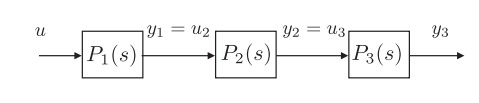
\includegraphics[width=\textwidth]{pictures/6_1.png} 
        \caption{Open-loop transfer
        function modeled as a cascade 流式 of
        three transfer functions.}
        \label{fig:6:1}
    \end{figure}
    \par 开环动力学由三个传递函数的乘积product给出: $P(s) = P_{1}(s)P_{2}(s)P_{3}(s)$.
    每一个传递函数都有一个输出$(y_{1}, y_{2}, y_{3})$, 该输出可以被测量和被用作反馈机制. Typically通常, 每个传递函数是是相对低阶的(low order, usually first or second order).
    在这个情形中,我们控制$y_{3}$输出, 而不是单独使用$y_{3}$反馈环, 我们将要连续使用$y_{1}, y_{2}, y_{3}$作为反馈机制, 如图\ref{fig:6:2}所示, 加入了三个自耦变压器(compensator) $C_{1}(s), C_{2}(s), C_{3}(s)$. 设计的一个必要条件是 内环控制要有最高的带宽, 每个连续环路带宽的频率最小要一秒$5 \sim 10$次。\par
    \begin{figure}[H]
        \centering % 图片居中
        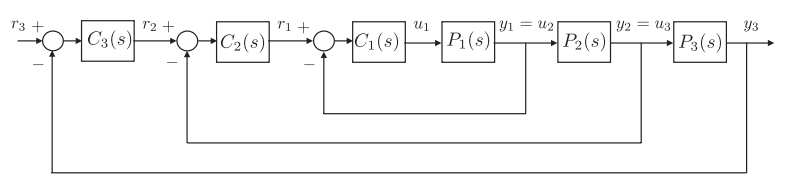
\includegraphics[width=\textwidth]{pictures/6_2.png} 
        \caption{three-stage successive loop closure design}
        \label{fig:6:2}
    \end{figure}
    \begin{figure}[htpb]
        \centering % 图片居中
        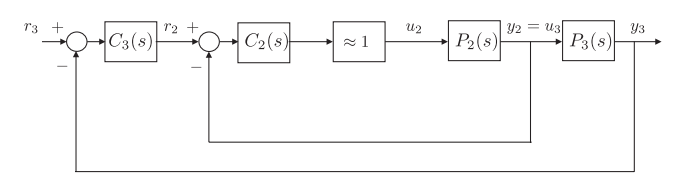
\includegraphics[width=\textwidth]{pictures/6_3.png} 
        \caption{Successive loop closure design with inner loop modeled as a unity
        gain}
        \label{fig:6:3}
    \end{figure}
    如图\ref{fig:6:2}, 目标是设计一个从$r_{1}$到$y_{1}$闭环系统, 带宽是$\omega_{BW1}$.
    关键的假设是频率远远低于$\omega_{BW1}$, 闭环控制传递函数$\frac{y_{1}(s)}{r_{1}(s)}$能被作为增益为1的模型, 如图\ref{fig:6:3}. 在内环传递函数增益为1的模型的情形下,设计第二个环路就简单了很多, 因为第二个环路仅仅包含了传递函数$P_{2}(s)$和自耦变压器$C_{2}(s)$. 
    连续环路的关键critical一步是设计下一个环路的带宽,使其比前一个环路小S倍,S通常是从5到10之间的取值. 此时,$\omega_{BW2} < \frac{1}{S} \omega_{BW1} $, 因此确保在中间环路工作的频率范围内, 不违反内部环路的单位增益假设.
    \par 两个内环设计之后, 对于最外层的设计, $\frac{y_{2}(s)}{r_{2}(s)} \approx 1 $ 并且从$r_{2}(s)$到$y_{2}(s)$的传递函数可以被收益为1代替, 如图\ref{fig:6:4}. 再一次设计外环控制带宽限制为 $\omega_{BW3} < \frac{1}{s_{2}} \omega_{BW2}$.
    因为每一传递函数 $P_{1}(s), P_{2}(s), P_{3}(s)$ 是一阶到二阶, 常规的PID或者滞后自耦变压器可以被有效的使用.通常使用基于传递函数的设计方法,例如根轨迹或循环成形方法。
    \begin{figure}[H]
        \centering % 图片居中
        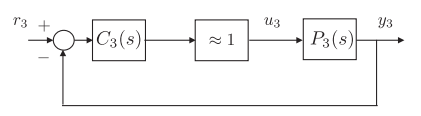
\includegraphics[width=\textwidth]{pictures/6_4.png} 
        \caption{Successive-loop-closure
        design with two inner loops modeled
        as a unity gain.}
        \label{fig:6:4}
    \end{figure}
    \par 以下各节讨论了横向自动驾驶仪和纵向自动驾驶仪的设计。建模横向和纵向动力学的传递函数在5.4节中开发,并将在本章中用于设计自动驾驶仪.
    \clearpage
    \section{Saturation Constraints and Performance 饱和约束和性能}
    连续的闭环的设计,意味着系统的性能受最内层循环性能的限制. 最内层循环经常被 saturation Constraints 饱和约束 所限制,  
    比如,在横向飞行器设计的时候, 机翼在其偏转角度烦方面有物理上的限制,从而导致了 roll 速率受限制. 
    所以,目标是去设计内层循环在不违反饱和约束性的情况下, 带宽尽可能的大. 并且设计外层循环来使得连续控制环的带宽分离. 
    在该节, 我们明确描述了 控制器传递函数和执行器饱和约束性能能被用来发展最内层循环控制的性能独特性. 
    使用一个二阶系统\ref{fig:6:5}来阐明这个处理.
    \par
    图\ref{fig:6:5}所示的二阶系统,其输出误差是比例反馈,输出微分反馈,则闭环传递函数为\ref{equ:1}. 可得, 闭环控制系统的极点(poles)被控制收益 $k_{p}$ 和 $k_{d}$ 所定义. 执行器工作量$u$可以被 $u = k_{p}e - k_{d}\dot{y}$ 所表示. 当 $\dot{y}$是0或者小的时候, 执行器工作量(actuator effort) $u$ 主要受到控制误差 $e$ 和 控制收益 $k_{p}$ 的影响, 如果系统是稳定的, the largest control effort in response to a step input will occur immediately after the step, where $u^{max} = k_{p}e^{max}$. 重新整理该公式,  可得 比例控制收益能被最大的预期输出误差和执行器的饱和约所决定. 整理得公式\ref{equ:2}, 其中 $u^{max}$ 是系统提供的最大控制工作量, $e^{max}$ 是步误差, 可以由标称尺寸的步进输入所导致. (paper 115 equation 6.3)
    \begin{equation}
        \frac{y}{y^{c}} = \frac{b_{0}k_{p}}{s^{2} + (a_{1} + b_{0}k_{d})s + (a_{0} + b_{0}k_{p})}
        \label{equ:1}
    \end{equation}
    \begin{figure}[H]
        \centering % 图片居中
        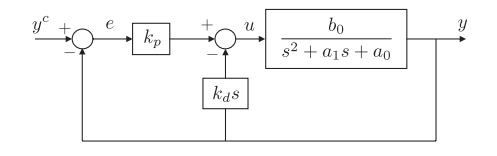
\includegraphics[width=\textwidth]{pictures/6_5.png} 
        \caption{Control System example}
        \label{fig:6:5}
    \end{figure}

    \begin{equation}
        k_{p} = \frac{u^{max}}{e^{max}}
        \label{equ:2}
    \end{equation}








    \clearpage

    \section{Lateral-directional Autopilot 横向自动驾驶仪}

    \subsection{Roll Attitude Loop Design }

    \subsection{Course Hold}

    \subsection{Sideslip Hold}

    \section{Longitudinal Autopilot}
    \subsection{Pitch Attitude Hold}

    \subsection{Altitude Hold Using Commanded Pitch}

    \subsection{Airspeed Hold Using Commanded Pitch}
    \subsection{Airspeed Hold Using Throttle}

    \subsection{Altitude-control State Machine}

    \section{Digital Implementation of PID Loops}


\end{document}